\documentclass{beamer}

\usepackage{amsmath}

\usetheme{AnnArbor}
\usecolortheme{crane}
\usefonttheme[onlymath]{serif}

\title{Deep Learning - Foundations and Concepts}
\subtitle{Chapter 16. Continuous Latent Variables}
\author{nonlineark@github}
\date{\today}

\begin{document}

\begin{frame}
    \titlepage
\end{frame}

\begin{frame}
    \frametitle{Outline}
    \tableofcontents
\end{frame}

\section{Principal Component Analysis}

\begin{frame}
    \frametitle{Maximum variance formulation}
    \begin{block}{Problem}
        Consider a data set of observations $\{x_{n}\}$ where $n=1,\hdots,N$, and $x_{n}$ is a Euclidean variable with dimensionality $D$. Our goal is to project the data onto a space having dimensionality $M<D$ while maximizing the variance of the projected data.
    \end{block}
\end{frame}

\begin{frame}
    \frametitle{Maximum variance formulation}
    Let's calculate the variance of the projected data on a unit direction $v$:
    \begin{align*}
        y_{n}&=x_{n}\cdot{}v \\
        E(y_{n})&=\frac{1}{N}\sum_{n=1}^{N}y_{n}=E(x_{n})\cdot{}v \\
        \mathrm{var}(y_{n})&=\frac{1}{N}\sum_{n=1}^{N}(y_{n}-E(y_{n}))^{2}=\frac{1}{N}\sum_{n=1}^{N}((x_{n}-E(x_{n}))\cdot{}v)^{2} \\
        &=\frac{1}{N}\sum_{n=1}^{N}v^{T}(x_{n}-E(x_{n}))(x_{n}-E(x_{n}))^{T}v=v^{T}Sv
    \end{align*}
    where $S$ is the data covariance matrix defined by:
    \begin{equation*}
        S=\frac{1}{N}\sum_{n=1}^{N}(x_{n}-E(x_{n}))(x_{n}-E(x_{n}))^{T}
    \end{equation*}
\end{frame}

\begin{frame}
    \frametitle{Maximum variance formulation}
    Let's find the unit direction $v_{1}$ for the largest variance. Suppose that $\lambda_{1}\ge\cdots\ge\lambda_{D}$ are the $D$ eigenvalues of $S$, and their corresponding orthonormal eigenvectors are $u_{1},\hdots,u_{D}$ respectively. Let $\Lambda=\mathrm{diag}(\lambda_{1},\hdots,\lambda_{D})$, $U=\begin{pmatrix}
        u_{1}&\cdots&u_{D}
    \end{pmatrix}$. We have:
    \begin{align*}
        v_{1}&=U\alpha_{1} \\
        v_{1}^{T}Sv_{1}&=\alpha_{1}^{T}U^{T}SU\alpha_{1}=\alpha_{1}^{T}\Lambda\alpha_{1}\le\lambda_{1}||\alpha_{1}||^{2}=\lambda_{1}
    \end{align*}
    The equality holds if and only if $v_{1}$ is an eigenvector corresponds to the largest eigenvalue $\lambda_{1}$. Without loss of generality, we could set $v_{1}=u_{1}$.
\end{frame}

\begin{frame}
    \frametitle{Maximum variance formulation}
    Let's find the unit direction $v_{2}$ for the second largest variance. Because $v_{2}$ is orthogonal to $v_{1}$ thus $u_{1}$, in the coordinate system formed by the orthonormal basis $u_{1},\hdots,u_{D}$, its first coordinate is $0$:
    \begin{align*}
        v_{2}&=U\alpha_{2} \\
        v_{2}^{T}Sv_{2}&=\alpha_{2}^{T}\Lambda\alpha_{2}\le\lambda_{2}||\alpha_{2}||^{2}=\lambda_{2}
    \end{align*}
    Again, the equality holds if and only if $v_{2}$ is an eigenvector corresponds to the second largest eigenvalue $\lambda_{2}$. Without loss of generality, we could set $v_{2}=u_{2}$.
\end{frame}

\begin{frame}
    \frametitle{Maximum variance formulation}
    If we consider the general case of an $M$-dimensional projection space, the optimal linear projection for which the variance of the projected data is maximized is now defined by the $M$ eigenvectors $u_{1},\hdots,u_{M}$ of the data covariance matrix $S$ corresponding to the $M$ largest eigenvalues $\lambda_{1},\hdots,\lambda_{M}$.
\end{frame}

\begin{frame}
    \frametitle{Minimum-error formulation}
    We now discuss an alternative formulation of PCA based on projection error minimization:
    \begin{itemize}
        \item We want to find an orthonormal basis $u_{1},\hdots,u_{D}$, where the $M$-dimensional linear subspace can be presented by the first $M$ of the basis vectors.
        \item Each data point $x_{n}$ is approximated by $\tilde{x}_{n}=\sum_{i=1}^{M}z_{ni}u_{i}+\sum_{i=M+1}^{D}b_{i}u_{i}$.
    \end{itemize}
    such that the squared distance between the original data point $x_{n}$ and its approximation $\tilde{x}_{n}$, averaged over the data set:
    \begin{equation*}
        J=\frac{1}{N}\sum_{n=1}^{N}||x_{n}-\tilde{x}_{n}||^{2}
    \end{equation*}
    is minimized.
\end{frame}

\begin{frame}
    \frametitle{Minimum-error formulation}
    \begin{align*}
        0&=\frac{\partial{}J}{\partial{}z_{ni}}=-\frac{2}{N}(x_{n}^{T}u_{i}-z_{ni})\implies{}z_{ni}=x_{n}^{T}u_{i} \\
        0&=\frac{\partial{}J}{\partial{}b_{i}}=-\frac{2}{N}\sum_{n=1}^{N}(x_{n}^{T}u_{i}-b_{i})\implies{}b_{i}=(E(x_{n}))^{T}u_{i} \\
        x_{n}-\tilde{x}_{n}&=\sum_{i=M+1}^{D}((x_{n}-E(x_{n}))\cdot{}u_{i})u_{i} \\
        J&=\frac{1}{N}\sum_{n=1}^{N}||x_{n}-\tilde{x}_{n}||^{2}=\sum_{i=M+1}^{D}u_{i}^{T}Su_{i}
    \end{align*}
\end{frame}

\begin{frame}
    \frametitle{Minimum-error formulation}
    We recognize that $J$ is the total variance of the projected data on the unit directions $u_{M+1},\hdots,u_{D}$. To minimize $J$, $u_{M+1},\hdots,u_{D}$ should be the eigenvectors corresponding to the smallest $D-M$ eigenvalues of $S$, and hence the eigenvectors defining the principal subspace are those corresponding to the $M$ largest eigenvalues.
\end{frame}

\begin{frame}
    \frametitle{Data compression}
    One application for PCA is data compression:
    \begin{equation*}
        \tilde{x}_{n}=\sum_{i=1}^{M}(x_{n}\cdot{}u_{i})u_{i}+\sum_{i=M+1}^{D}(E(x_{n})\cdot{}u_{i})u_{i}=E(x_{n})+\sum_{i=1}^{M}((x_{n}-E(x_{n}))\cdot{}u_{i})u_{i}
    \end{equation*}
    This represents a compression of the data set, because for each data point we have replaced the $D$-dimensional vector $x_{n}$ with an $M$-dimensional vector.
\end{frame}

\begin{frame}
    \frametitle{Data whitening}
    Suppose we have a data set of observations $\{x^{n}\}$ where $n=1,\hdots,N$, and $x^{n}$ is a Euclidean variable with dimensionality $D$. We often want to transform the data set to standardize certain of its properties. For example, making a linear re-scaling of the individual variables such that each variable has zero mean and unit variance:
    \begin{align*}
        \bar{x}_{d}&=\frac{1}{N}\sum_{n=1}^{N}x^{n}_{d} \\
        \sigma^{2}_{d}&=\frac{1}{N}\sum_{n=1}^{N}(x^{n}_{d}-\bar{x}_{d})^{2} \\
        \tilde{x}^{n}_{d}&=\frac{x^{n}_{d}-\bar{x}_{d}}{\sigma_{d}}
    \end{align*}
\end{frame}

\begin{frame}
    \frametitle{Data whitening}
    The covariance matrix for the standardized data has components:
    \begin{equation*}
        \rho_{ij}=E(\tilde{x}^{n}_{i}\tilde{x}^{n}_{j})-E(\tilde{x}^{n}_{i})E(\tilde{x}^{n}_{j})=\frac{1}{N}\sum_{n=1}^{N}\frac{x^{n}_{i}-\bar{x}_{i}}{\sigma_{i}}\frac{x^{n}_{j}-\bar{x}_{j}}{\sigma_{j}}
    \end{equation*}
    If two components $x_{i}$ and $x_{j}$ of the data are perfectly correlated, then $\rho_{ij}=1$, and if they are uncorrelated, then $\rho_{ij}=0$.
\end{frame}

\begin{frame}
    \frametitle{Data whitening}
    Using PCA we can make a more substantial normalization of the data to give it zero mean and unit covariance, so that different variables become decorrelated:
    \begin{align*}
        y^{n}&=\Lambda^{-\frac{1}{2}}U^{T}(x^{n}-\bar{x}) \\
        E(y^{n})&=0 \\
        E(y^{n}(y^{n})^{T})&=\frac{1}{N}\sum_{n=1}^{N}\Lambda^{-\frac{1}{2}}U^{T}(x^{n}-\bar{x})(x^{n}-\bar{x})^{T}U\Lambda^{-\frac{1}{2}} \\
        &=\Lambda^{-\frac{1}{2}}U^{T}SU\Lambda^{-\frac{1}{2}}=\Lambda^{-\frac{1}{2}}\Lambda\Lambda^{-\frac{1}{2}}=I \\
        \mathrm{cov}(y^{n})&=E(y^{n}(y^{n})^{T})-E(y^{n})(E(y^{n}))^{T}=I
    \end{align*}
\end{frame}

\begin{frame}
    \frametitle{High-dimensional data}
    In some applications of PCA, the number of data points is smaller than the dimensionality of the data space. For such cases, we can calculate the eigenvalues and eigenvectors more efficiently this way:
    \begin{itemize}
        \item Let $X=\begin{pmatrix}
            x_{1}-\bar{x}&\cdots&x_{N}-\bar{x}
        \end{pmatrix}^{T}$, then $S=\frac{1}{N}X^{T}X$.
        \item Calculate the eigenvalues and eigenvectors of $\frac{1}{N}XX^{T}$ instead, say $\frac{1}{N}XX^{T}v=\lambda{}v$.
        \item Then $\lambda$ is an eigenvalue of $S$ and $u=X^{T}v$ is an eigenvector of $S$.
        \begin{itemize}
            \item $\frac{1}{\sqrt{N\lambda}}u$ is the corresponding unit eigenvector (suppose $v$ is already a unit vector).
        \end{itemize}
    \end{itemize}
\end{frame}

\section{Probabilistic Latent Variables}

\begin{frame}
    \frametitle{Probabilistic PCA}
    PCA can also be expressed as the maximum likelihood solution of a probabilistic latent variable model, known as probabilistic PCA:
    \begin{itemize}
        \item A probabilistic PCA model represents a constrained form of a Gaussian distribution.
        \item We can derive an EM algorithm for PCA that is computationally efficient.
        \item The combination of a probabilistic model and EM allows us to deal with missing values in the data set.
        \item Mixtures of probabilistic PCA models can be formulated in a principled way and trained using the EM algorithm.
    \end{itemize}
\end{frame}

\begin{frame}
    \frametitle{Probabilistic PCA}
    \begin{itemize}
        \item The existence of a likelihood function allows direct comparison with other probabilistic density models.
        \item Probabilistic PCA can be used to model class-conditional densities and hence be applied to classification problems.
        \item A probabilistic PCA model can be run generatively to provide samples from the distribution.
        \item Probabilistic PCA forms the basis for a Bayesian treatment of PCA.
    \end{itemize}
\end{frame}

\begin{frame}
    \frametitle{Generative model}
    Probabilistic PCA is a simple example of the linear Gaussian framework:
    \begin{itemize}
        \item Introduce an explicit $M$-dimensional latent variable $z$ corresponding to the principal component subspace:
        \begin{itemize}
            \item $p(z)=\mathcal{N}(z;0,I)$.
        \end{itemize}
        \item The $D$-dimensional observed variable $x$ is conditioned on the value of the latent variable:
        \begin{itemize}
            \item $p(x|z)=\mathcal{N}(x;Wz+\mu,\sigma^{2}I)$, where $W\in\mathbb{R}^{D\times{}M}$ and $\mu\in\mathbb{R}^{D}$.
        \end{itemize}
        \item The probabilistic PCA model is an example of a naive Bayes model, as $p(x|z)=\prod_{d=1}^{D}\mathcal{N}(x_{d};W_{d}z+\mu_{d},\sigma^{2})$, where $W_{d}$ is the $d$th row of $W$.
        \item We can view the probabilistic PCA model from a generative viewpoint: $x=Wz+\mu+\epsilon$, where $z\sim\mathcal{N}(z;0,I)$ is an $M$-dimensional Gaussian latent variable, and $\epsilon\sim\mathcal{N}(\epsilon;0,\sigma^{2}I)$ is a $D$-dimensional Gaussian noise.
    \end{itemize}
\end{frame}

\begin{frame}
    \frametitle{Likelihood function}
    The marginal distribution is again Gaussian, and is given by:
    \begin{equation*}
        p(x)=\mathcal{N}(x;\mu,WW^{T}+\sigma^{2}I)=\mathcal{N}(x;\mu,C)
    \end{equation*}
    The predictive distribution $p(x)$ is governed by the parameters $\mu$, $W$ and $\sigma^{2}$. However, there is redundancy in this parameterization corresponding to rotations of the latent space coordinates.
\end{frame}

\begin{frame}
    \frametitle{Maximum likelihood}
    Given a data set $\{x_{n}\}$, the log likelihood function is given by:
    \begin{align*}
        L&=\sum_{n=1}^{N}\log{}p(x_{n}) \\
        &=-\frac{ND}{2}\log{}2\pi-\frac{N}{2}\log\det{}C-\frac{1}{2}\sum_{n=1}^{N}(x_{n}-\mu)^{T}C^{-1}(x_{n}-\mu)
    \end{align*}
    It's easy to maximize $L$ with respect to $\mu$:
    \begin{equation*}
        0=\frac{\partial{}L}{\partial\mu}=\sum_{n=1}^{N}(x_{n}-\mu)^{T}C^{-1}\implies\mu_{ML}=\frac{1}{N}\sum_{n=1}^{N}x_{n}=\bar{x}
    \end{equation*}
\end{frame}

\begin{frame}
    \frametitle{Maximum likelihood}
    Maximization with respect to $W$ and $\sigma^{2}$ is more complex but nonetheless has an exact closed-form solution:
    \begin{align*}
        \sigma^{2}_{ML}&=\frac{1}{D-M}\sum_{i=M+1}^{D}\lambda_{i} \\
        W_{ML}&=U_{M}(\Lambda_{M}-\sigma^{2}_{ML}I)^{\frac{1}{2}}R
    \end{align*}
    where:
    \begin{itemize}
        \item $\lambda_{1}\ge\cdots\ge\lambda_{D}$ are the eigenvalues of $S$.
        \item $u_{1},\hdots,u_{D}$ are the corresponding eigenvectors of $S$.
        \item $\Lambda_{M}=\mathrm{diag}(\lambda_{1},\hdots,\lambda_{M})$.
        \item $U_{M}=\begin{pmatrix}
            u_{1}&\cdots&u_{M}
        \end{pmatrix}$.
        \item $R$ is an arbitrary $M\times{}M$ orthogonal matrix.
    \end{itemize}
\end{frame}

\begin{frame}
    \frametitle{Maximum likelihood}
    It is worth taking a moment to study the form of the covariance matrix $C$:
    \begin{equation*}
        C=W_{ML}W_{ML}^{T}+\sigma^{2}_{ML}I=U_{M}(\Lambda_{M}-\sigma^{2}_{ML}I)U_{M}^{T}+\sigma^{2}_{ML}I
    \end{equation*}
    Since the variance of the predictive distribution along some direction specified by the unit vector $v$ is given by $v^{T}Cv$, the variance along the direction of the eigenvectors is given by:
    \begin{equation*}
        u_{i}^{T}Cu_{i}=\begin{cases}
            (\lambda_{i}-\sigma^{2}_{ML})+\sigma^{2}_{ML}=\lambda_{i}&\textrm{if }1\le{}i\le{}M \\
            \sigma^{2}_{ML}&\textrm{if }M+1\le{}i\le{}D
        \end{cases}
    \end{equation*}
    In other words, this model correctly captures the variance of the data along the principal axes and approximates the variance in all remaining directions with a single average value $\sigma^{2}_{ML}$.
\end{frame}

\begin{frame}
    \frametitle{Maximum likelihood}
    The relation between probabilistic PCA and conventional PCA. The posterior distribution in latent space $p(z|x)$ is also a Gaussian:
    \begin{align*}
        p(z|x)&=\mathcal{N}(z;M^{-1}W_{ML}^{T}(x-\mu_{ML}),\sigma^{2}_{ML}M^{-1}) \\
        M&=W_{ML}^{T}W_{ML}+\sigma^{2}_{ML}I
    \end{align*}
    If we take the limit $\sigma^{2}_{ML}\to{}0$, then the posterior mean reduces to:
    \begin{equation*}
        (W_{ML}^{T}W_{ML})^{-1}W_{ML}^{T}(x-\bar{x})=R^{T}\Lambda_{M}^{-\frac{1}{2}}U_{M}^{T}(x-\bar{x})
    \end{equation*}
    which represents an orthogonal projection of the data point onto the latent space, and so we recover the standard PCA model.
\end{frame}

\begin{frame}
    \frametitle{Maximum likelihood}
    The probabilistic PCA model defines a multivariate Gaussian distribution in which the number of independent parameters can be controlled while still allowing the model to capture the dominant correlations in the data:
    \begin{itemize}
        \item The number of parameters scales quadratically with $D$ for the general Gaussian distribution.
        \item If we restrict the covariance matrix to be diagonal, then it can no longer express any correlations between them.
        \item For the probabilistic PCA model, the number of degrees of freedom in the covariance matrix $C$ is given by: $DM+1-\frac{M(M-1)}{2}$:
        \begin{itemize}
            \item The number of independent parameters in this model therefore only grows linearly with $D$, for fixed $M$.
            \item If we take $M=D-1$, then we recover the standard result for a full covariance Gaussian.
            \item If $M=0$, the model is equivalent to the isotropic covariance case.
        \end{itemize}
    \end{itemize}
\end{frame}

\begin{frame}
    \frametitle{Factor analysis}
    Factor analysis is a linear Gaussian latent variable model:
    \begin{align*}
        p(z)&=\mathcal{N}(z;0,I) \\
        p(x|z)&=\mathcal{N}(x;Wz+\mu,\Psi)
    \end{align*}
    where $\Psi=\mathrm{diag}(\psi_{1},\hdots,\psi_{D})$ is a $D\times{}D$ diagonal matrix.
\end{frame}

\begin{frame}
    \frametitle{Factor analysis}
    \begin{itemize}
        \item Factor analysis is an example of a naive Bayes model, as $p(x|z)=\prod_{d=1}^{D}\mathcal{N}(x_{d};W_{d}z+\mu_{d},\psi_{d})$, where $W_{d}$ is the $d$th row of $W$.
        \item As with probabilistic PCA, factor analysis is invariant to rotations in the latent space.
        \item Another difference between probabilistic PCA and factor analysis is their behavior under transformations of the data set:
        \begin{itemize}
            \item Probabilistic PCA is covariant under a rotation of the axes of the data space, since $R\sigma^{2}IR^{T}=\sigma^{2}I$.
            \item Factory analysis is covariant under component-wise re-scaling of the data variables, since $\Phi\Psi\Phi^{T}$ is still diagonal when $\Phi$ is diagonal.
        \end{itemize}
    \end{itemize}
\end{frame}

\begin{frame}
    \frametitle{Independent component analysis}
    In independent component analysis, the data variables are assumed to be linear mixtures of the latent variables, and the latent variables are assumed non-Gaussian and mutually independent:
    \begin{align*}
        p(z)&=\prod_{m=1}^{M}p(z_{m}) \\
        x&=Az
    \end{align*}
\end{frame}

\begin{frame}
    \frametitle{Kalman filters}
    \begin{figure}
        \caption{A linear dynamical system, or Kalman filter}
        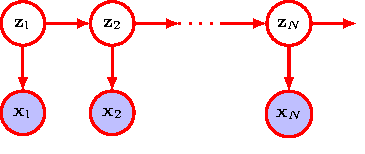
\includegraphics{Figure_9.pdf}
    \end{figure}
\end{frame}

\section{Evidence Lower Bound}

\begin{frame}
    \frametitle{Evidence lower bound}
    Consider a model $p(x,z;w)$ with an observed variable $x$, a latent variable $z$, and a learnable parameter vector $w$. If we introduce an arbitrary distribution $q(z)$ over the latent variable then we can write the log likelihood function $\log{}p(x;w)$ as:
    \begin{align*}
        \log{}p(x;w)&=\int{}q(z)\log\frac{p(x,z;w)}{q(z)}\mathrm{d}z-\int{}q(z)\log\frac{p(z|x;w)}{q(z)}\mathrm{d}z \\
        &=\mathcal{L}(q,w)+\mathrm{KL}(q(z)||p(z|x;w)) \\
        &\ge\mathcal{L}(q,w)
    \end{align*}
    we see that $\mathcal{L}(q,w)$ forms a lower bound on the log likelihood, known as the evidence lower bound or ELBO.
\end{frame}

\begin{frame}
    \frametitle{Evidence lower bound}
    We can maximize the log likelihood function using a two-stage iterative procedure called the expectation maximization algorithm, or EM algorithm:
    \begin{itemize}
        \item We first initialize the parameters $w^{(\textrm{old})}$.
        \item In the E step we keep $w^{(\textrm{old})}$ fixed and we maximize the lower bound with respect to $q(z)$:
        \begin{itemize}
            \item This is achieved when $q(z)=p(z|x;w^{(\textrm{old})})$ for which the Kullback-Leibler divergence is zero.
        \end{itemize}
        \item In the M step we keep this choice of $q(z)$ fixed and maximize $\mathcal{L}(q,w)$ with respect to $w$:
        \begin{itemize}
            \item This is equal to maximizing $\mathcal{Q}(w,w^{(\textrm{old})})=\int{}p(z|x;w^{(\textrm{old})})\log{}p(x,z;w)\mathrm{d}z$.
        \end{itemize}
    \end{itemize}
\end{frame}

\begin{frame}
    \frametitle{Evidence lower bound}
    For the particular case of i.i.d. data set, we have:
    \begin{align*}
        \mathcal{L}(q,w)&=\sum_{n=1}^{N}\int{}q(z_{n})\log\frac{p(x_{n},z_{n};w)}{q(z_{n})}\mathrm{d}z_{n} \\
        \mathcal{Q}(w,w^{(\textrm{old})})&=\sum_{n=1}^{N}\int{}p(z_{n}|x_{n};w^{(\textrm{old})})\log{}p(x_{n},z_{n};w)\mathrm{d}z_{n}
    \end{align*}
\end{frame}

\begin{frame}
    \frametitle{Expectation maximization}
    We can now use the EM algorithm to learn the parameters of the probabilitic PCA model:
    \begin{align*}
        p(z_{n})&=\mathcal{N}(z_{n};0,I)=\frac{1}{\sqrt{2\pi}^{K}}\exp(-\frac{1}{2}||z_{n}||^{2}) \\
        p(x_{n}|z_{n};W,\mu,\sigma^{2})&=\mathcal{N}(x_{n};Wz_{n}+\mu,\sigma^{2}I) \\
        &=\frac{1}{\sqrt{2\pi\sigma^{2}}^{D}}\exp(-\frac{1}{2\sigma^{2}}||x_{n}-Wz_{n}-\mu||^{2})
    \end{align*}
\end{frame}

\begin{frame}
    \frametitle{Expectation maximization}
    \begin{align*}
        \mathcal{Q}&=\sum_{n=1}^{N}E(\log{}p(z_{n})\log{}p(x_{n}|z_{n};W,\mu,\sigma^{2})) \\
        &=-\frac{NK}{2}\log{}2\pi-\frac{1}{2}\sum_{n=1}^{N}E(||z_{n}||^{2})-\frac{ND}{2}\log{}2\pi\sigma^{2} \\
        &\quad-\frac{1}{2\sigma^{2}}\sum_{n=1}^{N}E(||x_{n}-Wz_{n}-\mu||^{2}) \\
        &=-\frac{NK}{2}\log{}2\pi-\frac{1}{2}\sum_{n=1}^{N}\mathrm{tr}(E(z_{n}z_{n}^{T}))-\frac{ND}{2}\log{}2\pi\sigma^{2} \\
        &\quad-\frac{1}{2\sigma^{2}}\sum_{n=1}^{N}(||x_{n}-\mu||^{2}-2(x_{n}-\mu)^{T}WE(z_{n})+\mathrm{tr}(W^{T}WE(z_{n}z_{n}^{T})))
    \end{align*}
\end{frame}

\begin{frame}
    \frametitle{Expectation maximization}
    We already know that the exact maximum likelihood solution for $\mu$ is given by the sample mean $\bar{x}$. For the E step:
    \begin{align*}
        p(z_{n}|x_{n})&=\mathcal{N}(z_{n};M^{-1}W^{T}_{\textrm{old}}(x_{n}-\bar{x}),\sigma^{2}_{\textrm{old}}M^{-1}) \\
        M&=W^{T}_{\textrm{old}}W_{\textrm{old}}+\sigma^{2}_{\textrm{old}}I \\
        E(z_{n})&=M^{-1}W^{T}_{\textrm{old}}(x_{n}-\bar{x}) \\
        E(z_{n}z_{n}^{T})&=\mathrm{cov}(z_{n})+E(z_{n})(E(z_{n}))^{T}=\sigma^{2}_{\textrm{old}}M^{-1}+E(z_{n})(E(z_{n}))^{T}
    \end{align*}
\end{frame}

\begin{frame}
    \frametitle{Expectation maximization}
    For the M step:
    \begin{align*}
        0&=\frac{\partial\mathcal{Q}}{\partial{}W}(H)=\frac{1}{\sigma^{2}}\sum_{n=1}^{N}\mathrm{tr}((E(z_{n})(x_{n}-\bar{x})^{T}-E(z_{n}z_{n}^{T})W^{T})H) \\
        &\implies{}W=(\sum_{n=1}^{N}(x_{n}-\bar{x})(E(z_{n}))^{T})(\sum_{n=1}^{N}E(z_{n}z_{n}^{T}))^{-1} \\
        0&=\frac{\partial\mathcal{Q}}{\partial\sigma}=-\frac{ND}{\sigma}+\frac{1}{\sigma^{3}}\sum_{n=1}^{N}(||x_{n}-\bar{x}||^{2}-2(x_{n}-\bar{x})^{T}WE(z_{n}) \\
        &\qquad+\mathrm{tr}(W^{T}WE(z_{n}z_{n}^{T}))) \\
        &\implies\sigma^{2}=\frac{1}{ND}\sum_{n=1}^{N}(||x_{n}-\bar{x}||^{2}-2(x_{n}-\bar{x})^{T}WE(z_{n}) \\
        &\qquad+\mathrm{tr}(W^{T}WE(z_{n}z_{n}^{T})))
    \end{align*}
\end{frame}

\begin{frame}
    \frametitle{EM for PCA}
    We can take the limit $\sigma^{2}\to{}0$, corresponding to standard PCA. Let $X=\begin{pmatrix}
        x_{1}-\bar{x}&\cdots&x_{N}-\bar{x}
    \end{pmatrix}^{T}$ and $\Omega=\begin{pmatrix}
        E(z_{1})&\cdots&E(z_{N})
    \end{pmatrix}$, we have:
    \begin{align*}
        M&=W^{T}_{\textrm{old}}W_{\textrm{old}} \\
        \Omega&=M^{-1}W^{T}_{\textrm{old}}X^{T}=(W^{T}_{\textrm{old}}W_{\textrm{old}})^{-1}W^{T}_{\textrm{old}}X^{T} \\
        W&=X^{T}\Omega^{T}(\Omega\Omega^{T})^{-1}
    \end{align*}
\end{frame}

\begin{frame}
    \frametitle{EM for PCA}
    We see that:
    \begin{itemize}
        \item The E step involves an orthogonal projection of the data points onto the current estimate for the principal subspace.
        \item The M step represents a re-estimation of the principal subspace to minimize the reconstruction error in which the projections are fixed.
    \end{itemize}
\end{frame}

\begin{frame}
    \frametitle{EM for PCA}
    \begin{figure}
        \caption{Synthetic data illustrating the EM algorithm for PCA}
        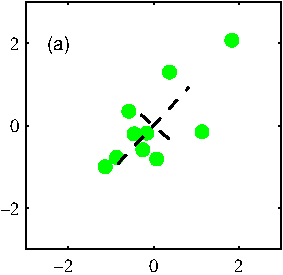
\includegraphics[width=0.25\textwidth]{Figure_10_a.pdf}
        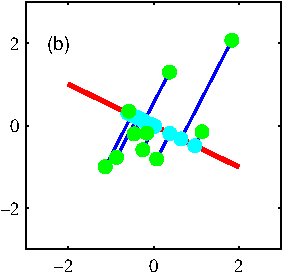
\includegraphics[width=0.25\textwidth]{Figure_10_b.pdf}
        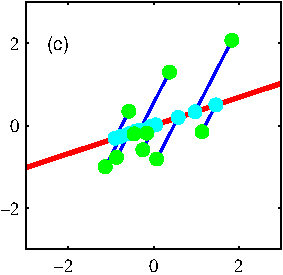
\includegraphics[width=0.25\textwidth]{Figure_10_c.pdf}
        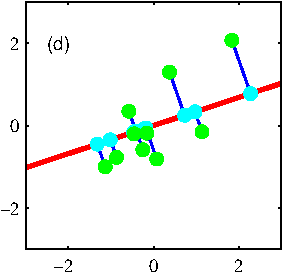
\includegraphics[width=0.25\textwidth]{Figure_10_d.pdf}
        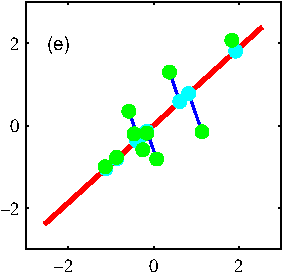
\includegraphics[width=0.25\textwidth]{Figure_10_e.pdf}
        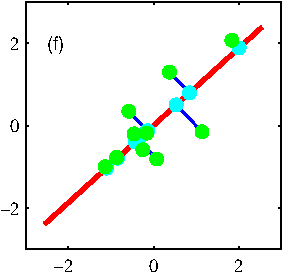
\includegraphics[width=0.25\textwidth]{Figure_10_f.pdf}
    \end{figure}
\end{frame}

\begin{frame}
    \frametitle{EM for factor analysis}
    We can also use the EM algorithm to learn the parameters of the factor analysis model:
    \begin{align*}
        &p(z_{n})=\mathcal{N}(z_{n};0,I)=\frac{1}{\sqrt{2\pi}^{K}}\exp(-\frac{1}{2}||z_{n}||^{2}) \\
        &p(x_{n}|z_{n};W,\mu,\Psi)=\mathcal{N}(x_{n};Wz_{n}+\mu,\Psi) \\
        &=\frac{1}{\sqrt{2\pi}^{D}}\frac{1}{\sqrt{\det\Psi}}\exp(-\frac{1}{2}(x_{n}-Wz_{n}-\mu)^{T}\Psi^{-1}(x_{n}-Wz_{n}-\mu))
    \end{align*}
\end{frame}

\begin{frame}
    \frametitle{EM for factor analysis}
    \begin{align*}
        \mathcal{Q}&=\sum_{n=1}^{N}E(\log{}p(z_{n})\log{}p(x_{n}|z_{n};W,\mu,\Psi)) \\
        &=-\frac{N(K+D)}{2}\log{}2\pi-\frac{1}{2}\sum_{n=1}^{N}\mathrm{tr}(E(z_{n}z_{n}^{T}))-\frac{N}{2}\log\det\Psi \\
        &\qquad-\frac{1}{2}\sum_{n=1}^{N}(x_{n}-\mu)^{T}\Psi^{-1}(x_{n}-\mu)+\sum_{n=1}^{N}(x_{n}-\mu)^{T}\Psi^{-1}WE(z_{n}) \\
        &\qquad-\frac{1}{2}\sum_{n=1}^{N}\mathrm{tr}(W^{T}\Psi^{-1}WE(z_{n}z_{n}^{T}))
    \end{align*}
\end{frame}

\begin{frame}
    \frametitle{EM for factor analysis}
    We already know that the exact maximum likelihood solution for $\mu$ is give by the sample mean $\bar{x}$. For the E step:
    \begin{align*}
        p(z_{n}|x_{n})&=\mathcal{N}(z_{n};M^{-1}(W^{T}_{\textrm{old}}\Psi^{-1}_{\textrm{old}}(x_{n}-\bar{x})),M^{-1}) \\
        M&=W^{T}_{\textrm{old}}\Psi^{-1}_{\textrm{old}}W_{\textrm{old}}+I \\
        E(z_{n})&=M^{-1}W^{T}_{\textrm{old}}\Psi^{-1}_{\textrm{old}}(x_{n}-\bar{x}) \\
        E(z_{n}z_{n}^{T})&=\mathrm{cov}(z_{n})+E(z_{n})(E(z_{n}))^{T}=M^{-1}+E(z_{n})(E(z_{n}))^{T}
    \end{align*}
\end{frame}

\begin{frame}
    \frametitle{EM for factor analysis}
    For the M step:
    \begin{align*}
        0&=\frac{\partial\mathcal{Q}}{\partial{}W}H=\sum_{n=1}^{N}\mathrm{tr}((E(z_{n})(x_{n}-\bar{x})^{T}-E(z_{n}z_{n}^{T})W^{T})\Psi^{-1}H) \\
        &\implies{}W=(\sum_{n=1}^{N}(x_{n}-\bar{x})(E(z_{n}))^{T})(\sum_{n=1}^{N}E(z_{n}z_{n}^{T}))^{-1} \\
        0&=\frac{\partial\mathcal{Q}}{\partial\Lambda}H=\frac{N}{2}\mathrm{tr}(\Psi{}H)-\frac{N}{2}\mathrm{tr}(SH)+\sum_{n=1}^{N}\mathrm{tr}(WE(z_{n})(x_{n}-\bar{x})^{T}H) \\
        &\qquad-\frac{1}{2}\sum_{n=1}^{N}\mathrm{tr}(WE(z_{n}z_{n}^{T})W^{T}H) \\
        &\implies\Psi=\mathrm{diag}(S-W\frac{1}{N}\sum_{n=1}^{N}E(z_{n})(x_{n}-\bar{x})^{T})
    \end{align*}
\end{frame}

\section{Nonlinear Latent Variable Models}

\begin{frame}
    \frametitle{Nonlinear latent variable models}
    We can use the flexibility of deep neural networks to represent more complex transformations from the latent space to the data space:
    \begin{align*}
        p_{z}(z)&=\mathcal{N}(z;0,I) \\
        x&=g(z;w)
    \end{align*}
    where $w$ represents the weights and biases.
\end{frame}

\begin{frame}
    \frametitle{Nonlinear latent variable models}
    For learning:
    \begin{itemize}
        \item The likelihood function is given by: $p_{x}(x)=p_{z}(z(x))|\det{}J(x)|$, where $J(x)=\frac{\partial(z_{1},\hdots,z_{D})}{\partial(x_{1},\hdots,x_{D})}$ is the Jacobian matrix.
        \item We need the inverse $z=g^{-1}(x;w)$ of the neural network function, but for most neural networks this inverse will not be well defined.
    \end{itemize}
    For sampling:
    \begin{itemize}
        \item Sampling from such a model is straightforward because we can generate samples from $p_{z}(z)$ and then transform each of them using the neural network function to give corresponding samples of $x$.
    \end{itemize}
\end{frame}

\begin{frame}
    \frametitle{Nonlinear manifolds}
    Consider the situation in which $z$ has dimensionality $M$ and $x$ has dimensionality $D$, where $M<D$. In this case the distribution over $x$ is confined to a manifold.
    \begin{figure}
        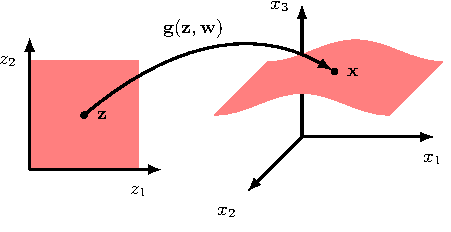
\includegraphics{Figure_11.pdf}
    \end{figure}
\end{frame}

\begin{frame}
    \frametitle{Nonlinear manifolds}
    However, this framework assigns zero probability density to any data vector that does not lie exactly on the manifold, which is a problem for gradient-based learning. To address this, we define a conditional distribution across the entire data space, whose parameters are given by the output of the neural network:
    \begin{align*}
        p(z)&=\mathcal{N}(z;0,I) \\
        p(x|z;w)&=\mathcal{N}(x;g(z;w),\sigma^{2}I)
    \end{align*}
    This is assuming that $x$ is a vector of continuous variables, and $g(z;w)$ has linear output-unit functions.
\end{frame}

\begin{frame}
    \frametitle{Nonlinear manifolds}
    \begin{figure}
        \caption{Illustration of a nonlinear latent-variable model for a one-dimensional latent space and a two-dimensional data space}
        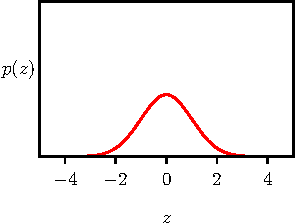
\includegraphics[height=0.4\textheight]{Figure_13_a.pdf}
        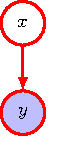
\includegraphics[height=0.4\textheight]{Figure_13_b.pdf}
    \end{figure}
\end{frame}

\begin{frame}
    \frametitle{Likelihood function}
    Now suppose we wish to fit the model to an observed data set by maximizng the likelihood function. One approach for evaluating the likelihood function would be to draw samples from the latent space distribution:
    \begin{equation*}
        p(x;w)=\int{}p(x|z;w)p(z)\mathrm{d}z=\frac{1}{K}\sum_{k=1}^{K}p(x|z_{k};w)
    \end{equation*}
    where $z_{k}\sim{}p(z)$. However, the value of $K$ needed for effective training will typically be far too high to be practical.
\end{frame}

\begin{frame}
    \frametitle{Discrete data}
    If the observed data set comprises independent binary variables then we can use a conditional distribution of the form:
    \begin{align*}
        p(x|z;w)&=\prod_{d=1}^{D}g_{d}(z;w)^{x_{d}}(1-g_{d}(z;w))^{1-x_{d}} \\
        g_{d}(z;w)&=\sigma(a_{d}(z;w))
    \end{align*}
\end{frame}

\begin{frame}
    \frametitle{Discrete data}
    For one-hot encoded categorical variables, we can use a multinomial distribution:
    \begin{align*}
        p(x|z;w)&=\prod_{d=1}^{D}g_{d}(z;w)^{x_d} \\
        g_{d}(z;w)&=\frac{\exp(a_{d}(z;w))}{\sum_{d'=1}^{D}\exp(a_{d'}(z;w))}
    \end{align*}
\end{frame}

\begin{frame}
    \frametitle{Four approaches to generative modelling}
    \begin{itemize}
        \item Nonlinear latent-variable models based on deep neural networks offer a highly flexible framework for building generative models.
        \item However, we have also identified some challenges associated with training such models that force us to develop more sophisticated techniques than those needed for linear models.
    \end{itemize}
\end{frame}

\begin{frame}
    \frametitle{Four approaches to generative modelling}
    \begin{itemize}
        \item Generative adversarial networks (GANs):
        \begin{itemize}
            \item Relax the requirement for the network mapping to be invertible.
            \item Abandon the concept of a likelihood function and instead introduce a second neural network whose function is to provide a training signal for the generative network.
        \end{itemize}
        \item Variational autoencoders (VAEs):
        \begin{itemize}
            \item Use a second neural network whose role is to approximate the posterior distribution over the latent variables.
        \end{itemize}
    \end{itemize}
\end{frame}

\begin{frame}
    \frametitle{Four approaches to generative modelling}
    \begin{itemize}
        \item Normalizing flows:
        \begin{itemize}
            \item The dimensionality of the latent space is set to be equal to that of the data space and the generative neural network is modified so that it becomes invertible.
            \item The likelihood function can be evaluated without approximation.
        \end{itemize}
        \item Diffusion models:
        \begin{itemize}
            \item Use a network that learns to transform a sample from the prior distribution into a sample from the data distribution through a sequence of denoising steps.
        \end{itemize}
    \end{itemize}
\end{frame}

\end{document}